\section{APPROACHES TO MULTIPLE OBJECTS TRANSPORTATION}
\subsection{Transformable Multirotor with Two-dimensional Multilink}
Zhao et al.\cite{Zhao2016} proposed a transformable multirotor comprising link modules with built-in propellers and achieved the stable aerial transformation. In other works\cite{ZhaoISER2016}\cite{ZhaoICRA2017}, they achieved the aerial manipulation by using the whole body of the transformable aerial robot. The joints with the same rotational axis allows the two-dimensional transformation as shown in \figref{multi_link}. In this work, we focus on the fact that this aerial robot possesses the ability to modify the CoG position actively. Thus, this aerial robot can keep the flight stable by aerial transformation although the number of objects it grasps changes. Therefore, using this way, we approach to the multiple objects transportation.
\begin{figure}[t]
  \begin{center}
    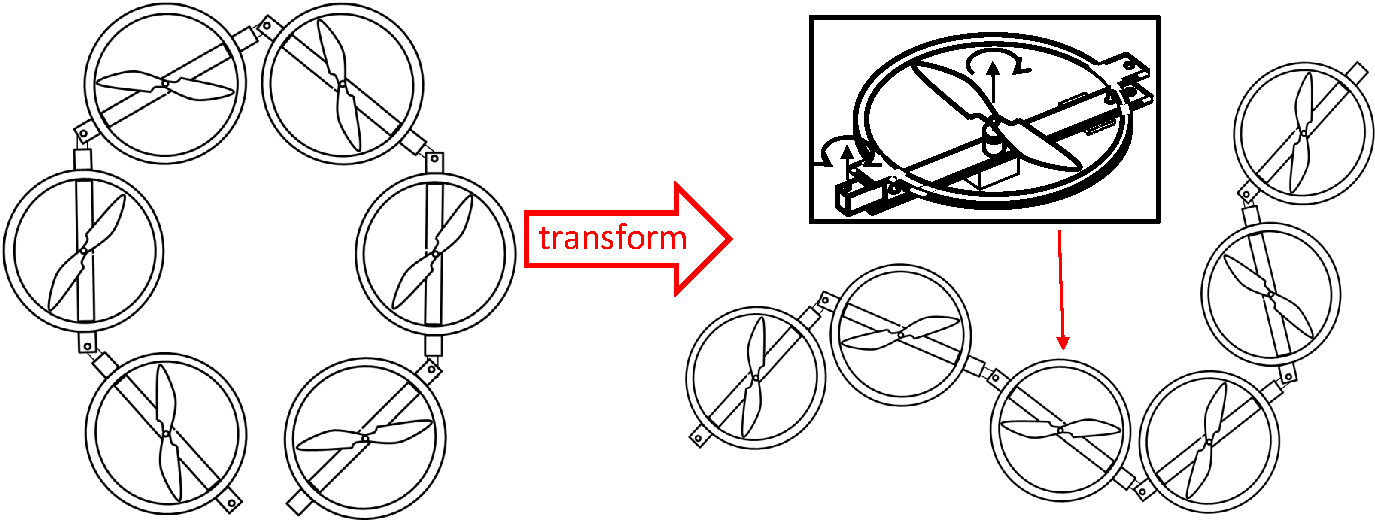
\includegraphics[width=1.0\columnwidth]{figs/multilink.pdf}
  \end{center}
  \caption{The structure and transformation of multirotor with multilinks. The multilinks consist of link modules.\label{figure:multi_link}}
\end{figure}
   
\subsection{Hardware Platform}
In previous works \cite{ZhaoISER2016}\cite{ZhaoICRA2017}\cite{Zhao2016}, quad-rotor with four-links was proposed and used in experiments. However, extension of the number of links was difficult due to the hardware structure: one central processor is connected to all actuators and sensors. Therefore, to extend the number of links, a novel structure of multilinks is necessary. For this reason, we construct a new link module which can be connected to each other easily. We also develop multi-drop structure for internal communication. Oung et al.\cite{Oung2010} proposed multi-propeller platform consisting of single-propeller modules and used infrared transceivers for communication of each single-propeller modules. However, it is considered that the communication speed with infrared transceivers is relatively low. Thus, we construct a wired network for communication of each link module. 

\subsection{Form Optimization Based on Flight Stability}
To keep the flight stable by aerial transformation, the multirotor with multilinks must transform to a particular form. In this work, to obtain the form, we propose the method of form optimization based on flight stability. In Sec. V, firstly, we investigate the definition of flight stability. Secondly, constraints of form considering the geometric condition and control stability are introduced. Finally, optimal forms are obtained by using gradient descent.
